\section{Entwicklungskonfiguration}
    \subsection{Hardware}

        \begin{center}
            \begin{tabular}{| l | l |}
                \hline
                Zweck & Hardware \\
                \hline
                Microkontroller & Atmega168PA \\
                \hline
                Sensor & MPU6050 \\
                \hline
                RGB-LED & HV-5RGBXX \\
                \hline
                UART & FTDI FT232RL\\
                \hline
                Programmer & MPLAB SNAP \\
                \hline
            \end{tabular}
        \end{center}

    \subsection{Software}

        \begin{center}
            \begin{tabular}{| l | l |}
                \hline
                Zweck & Software \\
                \hline
                IDE & MPLAB IDE v5.40 \\
                \hline
            \end{tabular}
        \end{center}


    \subsection{Inbetriebnahme}

        \subsubsection{Schaltplan}\label{schaltplan}
            Um die Kerze in Betrieb zu nehmen muss zunächst die
            Hardware aufgebaut werden. Dazu dient der folgende Schaltplan.
            \begin{figure}[H]
                \centering
                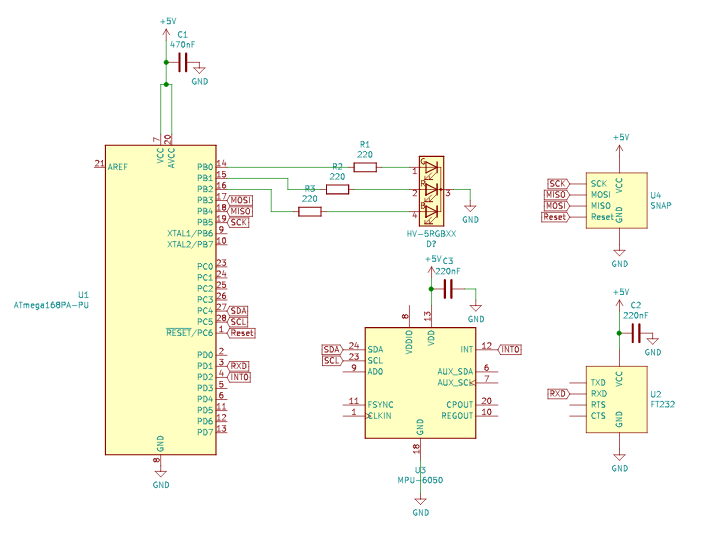
\includegraphics[scale=0.6]{img/schaltplan.png}
                \caption{Schaltplan}
            \end{figure}
            Hierbei ist zu beachten, dass der MPU6050 nicht durch seine Pins im
            Breakboard befestigt wird, sondern waagerecht aufgeklebt wird
            (Siehe \ref{Achsenorentierung}).

        \subsubsection{Kompilieren und Hochladen}
            Sobald die Hardware vollständig aufgebaut wurde, kann der
            \textit{MPLAB SNAP} Programmierer und das \textit{FT232} Modul,
            über Mikro-USB Kabel, an einen Computer angeschlossen werden und die
            \textit{MPLAB IDE} gestartet werden.
            Als nächstes muss das Projekt mit der \textit{MPLAB IDE} geöffnet werden.
            Der Programmer sollte erkannt werden und nach einem Klick auf
            \textit{Run} wird der Code kompiliert und auf die Hardware geladen.
            \\\\
            War dies erfolgreich, kann die Kerze wie im
            Benutzerhandbuch (Siehe \ref{Benutzerhandbuch}) beschrieben, genutzt
            werden.
